\documentclass[tikz,border=4pt]{standalone}
\usepackage[T1]{fontenc}
\usepackage{lmodern}
\renewcommand{\familydefault}{\sfdefault}
\usetikzlibrary{shapes.geometric,positioning,arrows.meta,calc,fit,backgrounds,decorations.pathreplacing}
\tikzset{
  node distance=6mm,
  every node/.style={font=\footnotesize,align=center,execute at begin node={\hyphenpenalty=10000\relax}},
  base/.style={draw=gray!60,fill=gray!12,minimum height=7mm,inner sep=2pt},
  term/.style={base,rounded corners=3.5mm,text width=30mm},
  proc/.style={base,text width=32mm},
  err/.style={base,text width=30mm,fill=gray!22},
  io/.style={base,trapezium,trapezium left angle=72,trapezium right angle=108,trapezium stretches=true,text width=28mm},
  dec/.style={base,diamond,aspect=2.4,text width=27mm,inner sep=0pt},
  % predefined process: a call to another procedure
  sub/.style={proc,inner xsep=3mm,path picture={
    \draw[gray!60] ([xshift=1.5mm]path picture bounding box.north west)--([xshift=1.5mm]path picture bounding box.south west)
                   ([xshift=-1.5mm]path picture bounding box.north east)--([xshift=-1.5mm]path picture bounding box.south east);}},
  go/.style={-{Stealth[length=2mm]},draw=gray!55!black},
  lab/.style={font=\scriptsize,fill=white,inner sep=1pt},
  frame/.style={draw=gray!60,dashed,rounded corners=2mm,inner sep=3mm},
  % memory diagrams
  cell/.style={draw=gray!60,fill=gray!12,minimum height=7mm,inner sep=1pt,font=\scriptsize},
  hot/.style={cell,fill=gray!35},
  note/.style={font=\scriptsize,text=gray!30!black},
}

\begin{document}
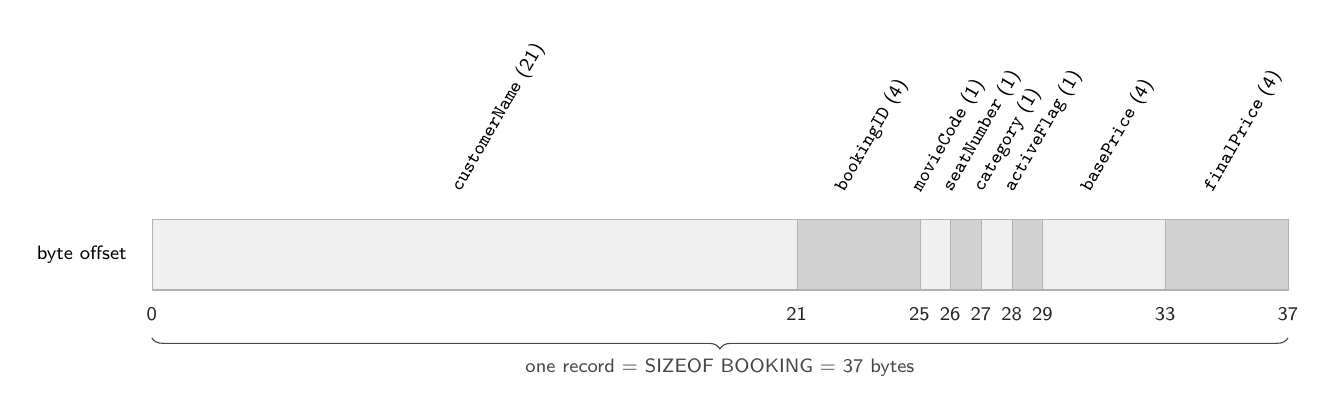
\begin{tikzpicture}[x=3.9mm,y=1mm]
% start offset / size / name / shade
\foreach \o/\s/\n/\st in {0/21/customerName/cell,21/4/bookingID/hot,25/1/movieCode/cell,26/1/seatNumber/hot,27/1/category/cell,28/1/activeFlag/hot,29/4/basePrice/cell,33/4/finalPrice/hot}{
  \node[\st,minimum width=\s*3.9mm,anchor=south west,minimum height=9mm] at (\o,0) {};
  \node[note,anchor=north] at (\o,-1) {\o};
  \node[anchor=south west,rotate=60,font=\scriptsize] at (\o+\s/2-0.2,10.5) {\texttt{\n} (\s)};
}
\node[note,anchor=north] at (37,-1) {37};
\draw[decorate,decoration={brace,mirror,amplitude=4pt},gray!55!black] (0,-6)--(37,-6) node[midway,below=4pt,font=\scriptsize]{one record = SIZEOF BOOKING = 37 bytes};
\node[font=\scriptsize,anchor=east] at (-0.5,4.5) {byte offset};
\end{tikzpicture}
\end{document}
